\section{Analysis}
\label{sec:Analysis}

The provided datasets consist of a Monte Carlo simulation of the $B^{\pm} \rightarrow K^{\pm} K^+ K^-$ decay channel and data recorded at the LHCb
experiment. The later one is reduced to relevant data by applying loose cuts on the given parameters. The provided parameters for both simulation
and real data are listed in the appendix. The simulated data does not include decays via resonances.\\

\subsection{Preselection}

To reduce combinatorial background and misidentified decays, tighter cuts on the given parameters are needed. By looking at the distributions of the
variables (\autoref{fig:ProbKPi}), that describe the likeliness of the hadron being a specific particle, one can decide for appropiate cuts. This is done for all three final state
hadrons. When choosing the cut, it is wise to not cut too tight. This would reduce signal events and worsen the statistics. Also, to ensure that the
hadrons are not muons, the variable \texttt{isMuon} is used for the preselection. The chosen cuts are listed
in \autoref{tab:Preselection}.
\begin{table}[h!]
  \centering
    \begin{tabular}{ |p{3cm}||p{3cm}|p{3cm}|p{3cm}|  }
      \hline
      \multicolumn{4}{|c|}{Preselection} \\
      \hline
      Variable & Hadron 1 &Hadron 2 &Hadron 3\\
      \hline
      \texttt{isMuon} (boolean)   & is not &is not&  is not\\
      \texttt{ProbK}&   $> 0.6$  &$> 0.55$   &$> 0.85$\\
      \texttt{ProbPi} & $< 0.3$ & $< 0.3$&  $< 0.3$\\

      \hline
      
    \end{tabular}
    \caption{The chosen cuts for the preselection of the recorded data. The values are chosen according to the distributions shown in \autoref{fig:ProbKPi}.}
    \label{tab:Preselection}
  \end{table}


 \begin{figure}
  \centering
  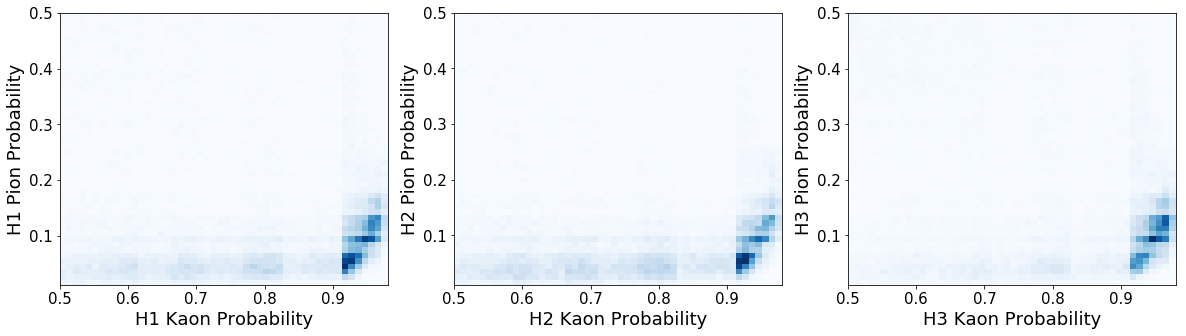
\includegraphics[width = .95\textwidth]{"content/pics/ProbKPi.png"}

  \caption{A 2-dimensional histogram for the Kaon and Pion Probability of the three hadrons.}
  \label{fig:ProbKPi}
\end{figure}
dawpidaiohih
\begin{figure}
  \centering
  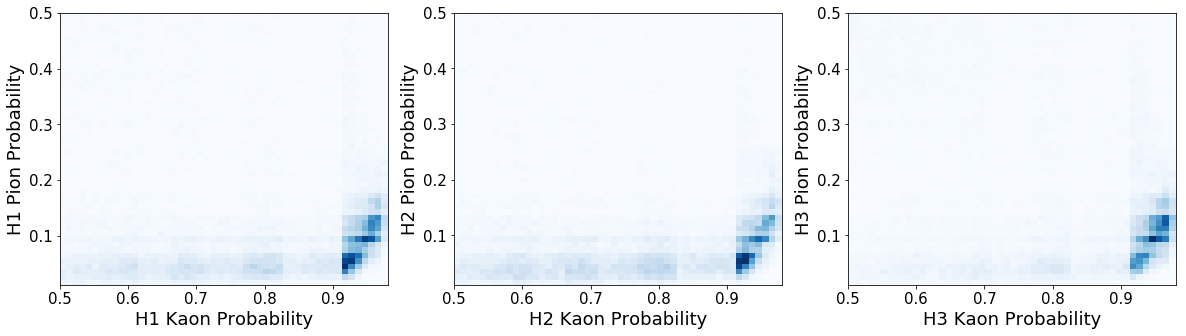
\includegraphics[width = .95\textwidth]{"content/pics/ProbKPi.png"}

  \caption{A 2-dimensional histogram for the Kaon and Pion Probability of the three hadrons.}
  \label{fig:ProbKPi}
\end{figure}